\documentclass[border=5pt]{standalone}
\usepackage{tikz}
\usetikzlibrary{calc}
\usepackage{amsmath}
\begin{document}
    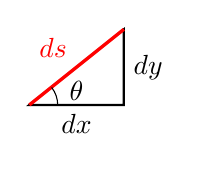
\begin{tikzpicture}[scale=1.2]
        % Draw the differential triangle
        \draw[thick] (0,0) -- (1,0) -- (1,0.8) -- cycle;

        \draw[very thick, red] (0,0) -- (1,0.8);

        % Label the sides
        \node[right] at (1,0.4) {$dy$};
        \node[below] at (0.5,0) {$dx$};
        \node[left, red] at (0.5,0.6) {$ds$};


        % Label the angle
        \draw (0.3,0) arc (0:38:0.3);
        \node at (0.5,0.15) {$\theta$};
    \end{tikzpicture}
\end{document}
